

%TODO
%
% #1 Expand to ECF?
% #2 Look chemistry of fat, glucose metabolism
% #3 BVP for weight loss
% #4 Use Mark's data
% #5 Fitbit steps to METs?
% 


\documentclass{article}[12pt]
\usepackage{graphicx, amsmath, amssymb,amsthm}
\usepackage[left=1in,right=1in,top=1in,bottom=1in]{geometry}
\usepackage{sidecap}

\oddsidemargin 0.25in
\evensidemargin 0.25in
\textwidth 6.0in

%\newtheorem{prob}{Exercise}[sect]
\newtheorem{theorem}{Theorem}[section]
\newtheorem{corollary}[theorem]{Corollary}
\newtheorem{lemma}[theorem]{Lemma}
\newtheorem{proposition}[theorem]{Proposition}
\newtheorem{remark}[theorem]{Remark}

\renewcommand{\labelenumi}{{\em(\roman{enumi}).}}


\title{On the Mathematics of Weight Loss}
\author{Jeffrey Humpherys}
\date{Partial Draft}
%\thanks{}
\begin{document}
\maketitle

%%%%%%%%%%%%%%%%%%%%%%%%%%%%%%%%%%%%%%%%%%%
%%%%%%%%%%%%%%%%%%%%%%%%%%%%%%%%%%%%%%%%%%%
%%%%%%%%%%%%%%%%%%%%%%%%%%%%%%%%%%%%%%%%%%%

\section{Introduction}

In 1997, the World Health Organization recognized obesity as a global epidemic \cite{PD,JLKS,HJ}, affecting one is six people in the world.  Among the most obesity-plagued countries is the United States, which, according to recent estimates by the Center for Disease Control \cite{FCOC}, claims one in three adults (33.8\%) and one in six children (17\%) \cite{OCCLF,MSDBM}.

Obesity is linked with numerous health problems such as high blood pressure, stroke, heart disease, type-2 diabetes, osteoarthritis, kidney disease, musculoskeletal disorders, sleep apnea, gallbladder disease, and several forms of cancer (e.g., endometrial, postmenopausal breast, kidney, and colon) \cite{FFW}.  In the U.S., obesity has become the second leading cause of preventative death, claiming 300,000 people per year \cite{AFMSV, FCOC}, and reducing life expectancy by 6-7 years on average, and by over 10 years in cases of extreme obesity \cite{PBWMAB,WLS}.

In addition to poor health and premature death, obesity also comes at a high cost financially.  As of 2008, the health care costs in the U.S. as a result of obesity have been estimated to be over \$147 billion annually, which represents over 9\% of national health care costs \cite{FTCD, FFW}.  According to the Society of Actuaries, the total annual cost of obesity in the U.S., which includes health care, disability, loss of productivity, etc., is \$270 billion \cite{SOA}.  Included in this estimate are consumer markets for diet, weight loss, and exercise, which are estimated to be at least \$40 billion \cite{Cu}.

It is important to note that despite the ever-expanding attention and effort toward weight loss, few interventions are successful in the long run, and the obesity epidemic continues to worsen.  While many diet and exercise programs enjoy short-term success, studies indicate that the majority individuals start to regain their weight within a few months.  In fact, it is estimated that only 20\% of those who lose more than 10\% of their weight are able to maintain their new weight for one year or more \cite{Wing2}.  Instead, most dieters experience \emph{weight cycling}, where weight is repeatedly lost and gained \cite{Wadden}.  Some recent studies suggest that it may be harder to keep the weight off than it is to lose it in the first place \cite{Co}.

So what are the keys to avoiding weight cycling and enjoying long-term success?  Some scholars suggest that the reason why so many people re-gain lost weight is that they revert to their previous lifestyle, and their heavier weight is just a consequence of that lifestyle \cite{BG}.  However, several leading studies link hormones such as leptin as major factor \cite{Keim,Ahima, Rosen,Fried}.

Leptin is a hormone produced by fat cells and released into the blood stream.  When someone loses body fat, their leptin levels drop, thus triggering a starvation response in the brain, and resulting in a desire to increase food intake and conserve energy \cite{Keim}.  In other words, when people lose fat, there is a strong natural instinct to restore it.  Through functional MRI (fMRI) studies, it has been shown that those with recently reduced leptin levels have greater cravings and hunger responses when shown images of food, particularly calorie-rich and high-fat foods \cite{Ahima, Rosen}.  This makes it all the more difficult to maintain a lower weight.  Leptin is also tied to satiation.  In studies where leptin-reduced subjects had their leptin levels increased through hormone therapy, appetite and hunger signals were normal.  Since these leptin responses appear in other mammals, scientists have suggested that these responses to leptin are a natural evolutionary instinct to fatten up after significant fat loss \cite{Fried}.  Other hormones, such as ghrelin, are also tied to weight loss, hunger, appetite, and certain food-related impulses.  Overall there are many complex interactions that take place, but one thing is clear: the body is naturally resistant to weight loss.

So, are our weight loss efforts in vain?  Perhaps not.  Scholars have recently examined the long-term behaviors from over 10,000 participants in the U.S. National Weight Control Registry ({\tt www.nwcr.ws}) who have lost 30 pounds or more and kept it off for more than a year.   Although this group is a self-selected pool of participants, and therefore the results do not hold up to the standards of a rigorous scientific study, over 90\% of respondents reported that they engaged in regular and rigorous physical exercise \cite{Wing1}.  This observation is consistent with recent studies that suggest that physical exercise counters the appetite-inducing and energy-conserving affects of leptin reduction \cite{Mac}.  In other words, leptin-reduced subjects who exercise regularly do not appear to experience the same cravings and lethargy as the more sedentary dieters.  Therefore, exercise may prove to be a critical component of a successful weight management program, not just as a way to burn extra calories but perhaps more importantly as the key to tempering appetite and boosting energy.  

Many respondents in the long-term weight control study also indicated that their diet-induced cravings subsided after a year.  This suggests that the affects of leptin reduction and other hormones are only temporary, and that the body will establish a new baseline for satiation over time.

Given the body's starvation response to rapid weight loss, an alternative weight management strategy has been proposed.  Rather than the standard two-phase approach of relatively short-term weight loss and long-term maintenance thereafter, some scholars have considered instead the strategy of ratcheting down to a desired weight by making small incremental lifestyle changes that are lasting \cite{Hill.2,Lutes}.  For example, every few weeks one would introduce another healthy habit, e.g., stop drinking sugar-laden soft drinks, replace certain foods with whole-grains, cut out certain snacks, drink more water, take the stairs instead of the elevator at work, park farther way from the office, or go on walks with co-workers and friends at lunchtime, etc.  This \emph{small changes} approach to diet and exercise may prove to be more sustainable and thus provide better success in the long-run.  The key to this strategy is that lasting weight loss requires long-term changes in behavior and lifestyle.  This process is slow and steady.  Moreover, by avoiding crash diets, the affects of leptin reduction and other hormones may be mitigated, thus curtailing somewhat the body's natural appetite and lethargy response to (perceived) starvation.  In other words, by losing weight slowly, there is hope that individuals will have greater long-term success than if they lose weight quickly.

Regardless of whether one uses rigorous exercise or small changes as their long-term weight management strategy, it is important have accurate expectations about how much one will lose, given the sacrifices and lifestyle changes that one makes.  Many failed dieters report that they quit dieting altogether because they got frustrated with their results.  The purpose of this paper is to examine weight change from a modern mathematical standpoint, where the dynamics of exercise and nutrition, when properly accounted, will dictate accurately a subject's weight over time.

%%%%%%%%%%%%%%%%%%%%%%%%%%%%%%%%%%%%%%%%%%%
%%%%%%%%%%%%%%%%%%%%%%%%%%%%%%%%%%%%%%%%%%%
%%%%%%%%%%%%%%%%%%%%%%%%%%%%%%%%%%%%%%%%%%%

\section{Background}

In this section, we examine some of the basic concepts behind the science of weight change that has evolved over the last century \cite{HB}.  In particular, we review standard caloric charts and indicators used in textbooks and weight management programs throughout the world.  We then describe how weight management advice can be tailored to an individual by replacing these population-based charts and formulae with personalized biometric measurements that can be taken at a doctor's office, pharmacy, weight management center, or gym.

Conventional wisdom equates a pound of fat with 3500 calories of body energy.  Hence, if you eat 200 calories per day over your recommended daily allowance, then accordingly you should gain a bit over 20 pounds in a year.  This logic breaks down when you consider eating an extra 200 calories per day for 20 years, which would amount to a gain of 400 lbs.  In reality, eating 200 calories per day over your recommended daily allowance would result in a long-term gain of roughly 25-35 pounds, depending on your body makeup.  In other words, if you eat a fixed number of calories on average each day over your recommended daily allowance your weight will saturate to a fixed amount over time---you don't keep gaining weight in perpetuity.  This is because as one gains weight, their metabolism goes up and they expend more energy moving their heavier body around.  Below we describe the predictive equations that determine this process.

The basic idea behind weight change is simple.  If ones energy intake is more than their energy expended, then they gain weight.  If their intake is less, then they lose weight.  The questions remain, ``how much can I eat each day on average and not lose weight?''  and ``how much should I eat if I want to achieve a goal weight''.  The textbook answers to these questions are given by the following recipe:
\begin{enumerate}
\item Determine your \emph{body mass index} (BMI) by taking your weight (W) in kilograms and dividing it by the square of your height (H) in meters, that is,
\begin{equation}
\label{BMI}
BMI = \dfrac{W}{H^2}.
\end{equation}
To convert from pounds to kilograms, divide the number of pounds by 2.2.  Thus 160 lbs. is 150/2.2=72.7 kilograms.  To convert from inches to meters, divide by 39.4.  Thus if a person is 5 feet, 8 inches tall (5'8'') or 68 inches, then they are 68/39.4 = 1.73 meters tall.  Thus a person who is 5'8'' and weighs 160 lbs has a BMI of 24.3 $kg/m^2$.
\item Determine your \emph{resting metabolic rate} (RMR) by taking your gender, age (A) in years, and height (H) from above, and using the formula:
\begin{equation}
\label{RMR}
RMR = \begin{cases} 9.99 W + 625 H + 5 A + 5 & \mbox{if male}\\ 9.99 W + 625 H + 5 A -161 & \mbox{if female.}\end{cases}
\end{equation}
For a 38 year old female who is 5'8'' and weighs 160 lbs, her estimated RMR according to \eqref{RMR} is 1459.6 calories per day.  We remark that there are several formulae given the literature for RMR; see \cite{HB, Mif, Fr}, however, \eqref{RMR} is the most widely used in the literature and is called the Mifflin equation.  We also note that \eqref{RMR} is an estimate based on a population study.  More accurate measurements of RMR can be performed by an indirect calorimetry device \cite{Fer}.
\item Determine your \emph{physical activity level} (PAL) by using the table below:
\begin{table}[h]
\label{PAL_table}
\begin{center}
\begin{tabular}{|l|l|}
\hline
1.40--1.69 & People who are sedentary and do not exercise regularly, spend \\
& most of their time sitting, standing, with little body displacement
\\
\hline
1.70--1.99 & People who are active, with frequent body displacement throughout  \\
& the day or who exercise frequently\\
\hline
2.00--2.40 & People who engage regularly in strenuous work or exercise for \\
& several hours each day\\
\hline
\end{tabular}
\caption{This is a rough guide for physical activity level (PAL).  For more detailed estimates, see \cite{Heym} and Appendix \ref{PAL_appendix}.}
\end{center}
\end{table}

\item Compute your energy expenditure (EE) using the formula:
\begin{equation}
\label{EE0}
EE = PAL \times RMR.
\end{equation}
This is the answer to the first question, ``how much can I eat each day on average and not lose weight?''  Thus, a sedentary 38 year old woman who weighs 160 pounds and is 5'8'' will burn $1.4 \times 1459.6 =2042.6$ calories each day on average.
\item Finally, determine your desired weight, compute the energy that you would expend at your desired weight.  That will give you the number of calories that you need to expend through increased exercise or decreased intake once you have achieved your desired weight.  However if you simply cut out the difference, it will take a very long time to achieve your desired weight.  Instead, many diet experts recommend that you reduce your calories by 10-25\% from your current EE until you reach your desired weight, noting that your EE will go down as you lose weight.  Thus, one may need to recompute their EE a few times along the way and adjust accordingly.
\end{enumerate}

\begin{remark}  Normal weight range is classified as having an BMI between 19.5 and 25.  A person is said to be overweight if their BMI is over 25, and obese if their BMI is over 30.  The woman in our example has an BMI of $24.3$.  This is on the high side of the normal weight range, and although she is not considered overweight, she may want to reduce her weight until her BMI is at the low end of the normal range, say to 20.6, or rather 136 lbs.
\end{remark}

We note that the recipe in the previous section represents the textbook approach to weight management.  These answers rely on several generalizations and assumptions taken from population studies, and are not tailored to an individual's body type and lifestyle.  Specifically, there are some significant deficiencies to this approach such as:
\begin{enumerate}
\item The Mufflin formula for RMR is based on population studies, and does not account for individual body types.  RMR can be measured specifically on an individual through a 10 minutes breathing test that uses indirect calorimetry to determine the amount of oxygen consumed while sitting down calmly.  Since oxygen is consumed in the body's metabolic processes, the amount of metabolized energy released in the form of heat can be determined.
\item PAL is a rough estimate on physical activity; to get a better estimate, see Appendix \ref{PAL_appendix}
\item BMI is a blunt way to determine ones ideal weight range.  Moreover it has been shown that the guidelines on obesity that use BMI need to be adjusted for race.\footnote{Recent studies suggest that the definition of obesity should be adjusted for Asians, and possibly other races where body sizes are proportioned differently on average \cite{Bei, Kan}.}
\item The time-frame required to lose weight is very unclear in this recipe.  The benefit of the dynamic approach, described below, is that one can estimate how long it will take to lose the desired weight, with a given weight management plan.  This is important because it will help alleviate frustration and thus reduce attrition.
\end{enumerate}

%%%%%%%%%%%%%%%%%%%%%%%%%%%%%%%%%%%%%%%%%%%
%%%%%%%%%%%%%%%%%%%%%%%%%%%%%%%%%%%%%%%%%%%
%%%%%%%%%%%%%%%%%%%%%%%%%%%%%%%%%%%%%%%%%%%

\section{A Dynamic Model of Human Body Weight Change}

In this section, we examine weight change from the point of view of thermodynamics and kinematics.  Weight change occurs when a ones energy balance is nonzero. Let \emph{energy balance}, denoted $EB$, be the difference between \emph{energy intake} $EI$ and \emph{energy expenditure} $EE$, that is,
\begin{equation}
\label{EB}
EB = EI - EE.
\end{equation}
When the energy intake exceeds the energy expended, the balance is positive and weight is gained.  Correspondingly, if the amount of energy expended exceeds the energy intake, the balance is negative and weight is lost.  Now, decomposing the different ways that energy is expended, we write
\begin{equation}
\label{EE}
EE = \underbrace{\delta BW}_\text{\parbox{1cm}{physical\\activity}} + \underbrace{\beta_{tef} EI}_\text{\parbox{1cm}{thermic\\effect of\\eating}} + \underbrace{\beta_{at} EI + \gamma_F F + \gamma_L L + \eta_F \dfrac{dF}{dt} + \eta_L \dfrac{dL}{dt}  + K}_\text{resting metabolic rate (RMR)},
\end{equation}
where $\gamma_F = 22$ kcal/kg/d, $\gamma_L = 3.2$ kcal/kg/d, $\eta_F = 180$ kcal/kg, and $\eta_L = 230$ kcal/kg; see \cite{Hall.2, Hall.4}.  Further, we let $\beta_{tef}=0.10$ and $\beta_{at}=0.14$ denote the coefficients for the thermic effect of feeding and adaptive thermogenesis, respectively.  The parameter $\delta$ is the coefficient representing the amount of energy expended from physical activity per kilogram of body mass.  Notice that $\gamma_L$ is significantly larger than $\gamma_F$.  This means that lean tissue metabolizes energy much faster than fatty tissue.  As a result, there are instances where one may want to increase their lean body mass through resistance training so that they are better able to support a higher caloric intake without significant weight gain.  Finally, we remark that the constant $K$ can be tuned to an individual's body type directly through RMR and fat measurement, and is assumed to remain constant over time.

Let $p(t)$ be the proportion of the energy balance that contributes to a gain or loss in lean tissue, and thus correspondingly $1-p(t)$ is the proportion of the energy balance that contributes to a gain or loss in fatty tissue.  Thus, we have the following compartmental model \cite{W,CH.1}:
\begin{subequations}
\label{compartment}
\begin{align}
\rho_F \dfrac{dF(t)}{dt} &= (1-p(t)) EB(t),\label{compartment:a}\\
\rho_L \dfrac{dL(t)}{dt} &= p(t) EB(t),\label{compartment:b}
\end{align}
\end{subequations}
where $\rho_F = 9400$ kcal/kg and $\rho_L = 1800$ kcal/kg are, respectively, the energy densities of fat and lean tissue.  Notice that the energy density of fat is much higher than the energy density of lean tissue.  Indeed fat is very energy rich; a pound of butter contains many more calories than a pound of beef.  

To close the equations in \eqref{compartment}, we determine how the proportionality constant $p$ varies with $F$ and $L$.  From Forbes' Law \cite{Fo.2}, we have that
\begin{equation}
\label{Forbes}
\dfrac{dF}{dL} = \dfrac{F}{10.4}.
\end{equation}
Hence,
\[
\dfrac{F}{10.4} = \dfrac{dF}{dL} = \dfrac{dF/dt}{dL/dt} = \dfrac{\dfrac{(1-p(t)) EB(t)}{\rho_F}}{\dfrac{p(t) EB(t)}{\rho_L}} = \dfrac{\rho_L}{\rho_F} \dfrac{1-p(t)}{p(t)}.
\]
Solving for $p(t)$ gives Forbes' equation
\begin{equation}
\label{Forbes2}
p(t) = \dfrac{C}{C+F(t)}\quad\mbox{where}\quad C=10.4\dfrac{\rho_L}{\rho_F}.
\end{equation}
Thus, since the input $EI$ is assumed to be known, we can use \eqref{EE} and \eqref{Forbes2} to write \eqref{compartment} in terms of $F$ and $L$, thus allowing us to close the system of ordinary differential equations (ODEs).  Specifically, we have
\begin{align*}
RMR(t) &= K + \gamma_F F(t) + \gamma_L L(t) + \eta_F \dfrac{dF}{dt} + \eta_L \dfrac{dL}{dt}  + \beta_{at} EI\\
&= K + \gamma_F F(t) + \gamma_L L(t) + \dfrac{\eta_F}{\rho_F} (1-p(t)) EB(t) + \dfrac{\eta_L}{\rho_L} p(t) EB(t)  + \beta_{at} EI.
\end{align*}
Thus,
\[
\left(\dfrac{1}{PAL}-\beta_{at}\right) EI = K + \gamma_F F(t) + \gamma_L L(t) + \left(\dfrac{\eta_F}{\rho_F} (1-p(t)) + \dfrac{\eta_L}{\rho_L} p(t) + \dfrac{1}{PAL}\right) EB(t).
\]
Solving for $EB(t)$, yields
\begin{equation}
\label{EB2}
EB(t) = \dfrac{\left( \dfrac{1}{PAL} - \beta_{at} \right) EI - K - \gamma_F F(t) - \gamma_L L(t)}{\dfrac{\eta_F}{\rho_F} (1-p(t)) + \dfrac{\eta_L}{\rho_L} p(t) + \dfrac{1}{PAL}}.
\end{equation}
To find, $K$, we note that
\begin{equation}
\label{K}
K = \left(\dfrac{1}{PAL}-\beta_{at}\right) EI - \gamma_F F(t) - \gamma_L L(t) - \eta_F \dfrac{dF}{dt} - \eta_L \dfrac{dL}{dt}  - \dfrac{1}{PAL} EB.
\end{equation}
In equilibrium, this is
\begin{equation}
\label{K2}
K = \left(\dfrac{1}{PAL}-\beta_{at}\right) EI - \gamma_F F - \gamma_L L.
\end{equation}
Thus, for a subject who has maintained the same weight for a while, one can determine $K$ by using \eqref{K2}, if they know their average caloric intake and amount of fat (assume $L=BW-F$).  

\begin{figure}[t]
\begin{center}%$
%\begin{array}{lr}
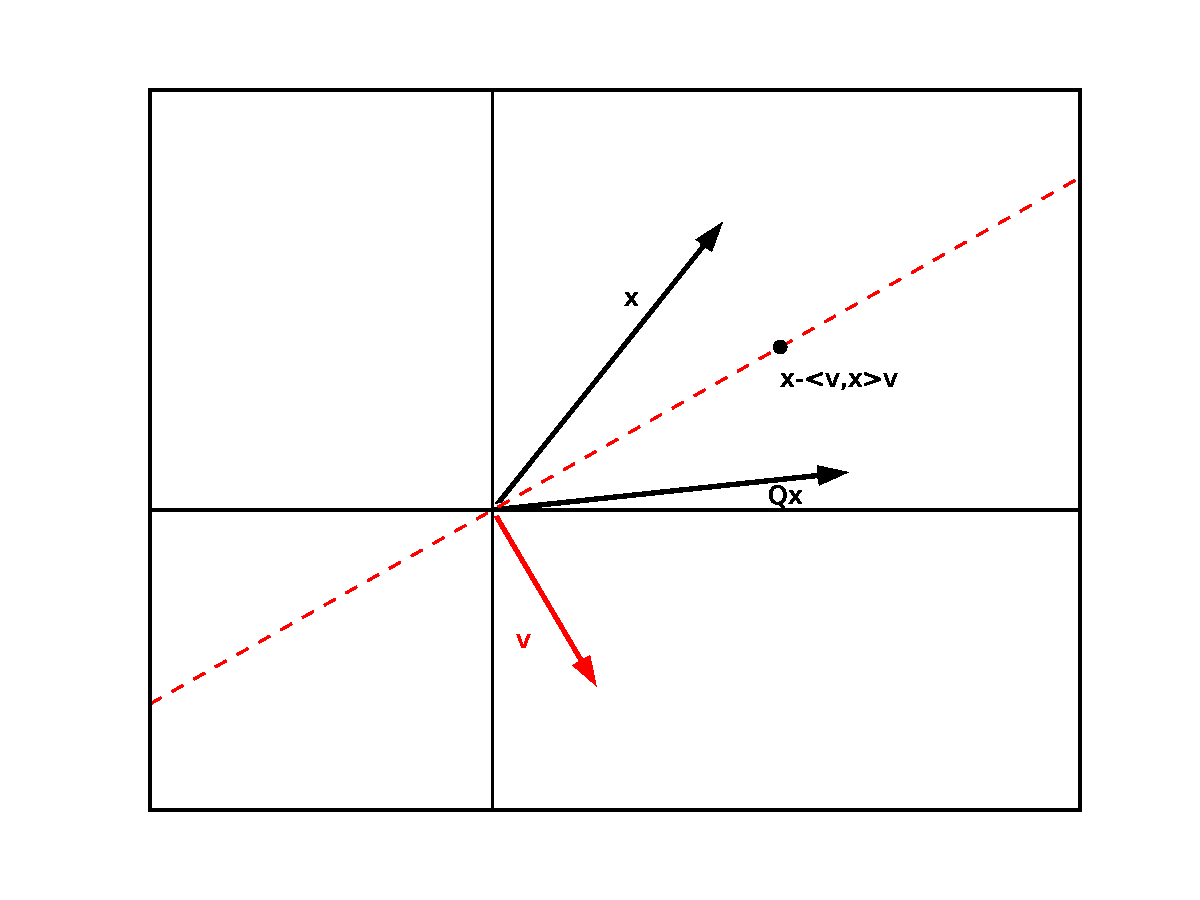
\includegraphics[width=12cm]{fig1} %&
%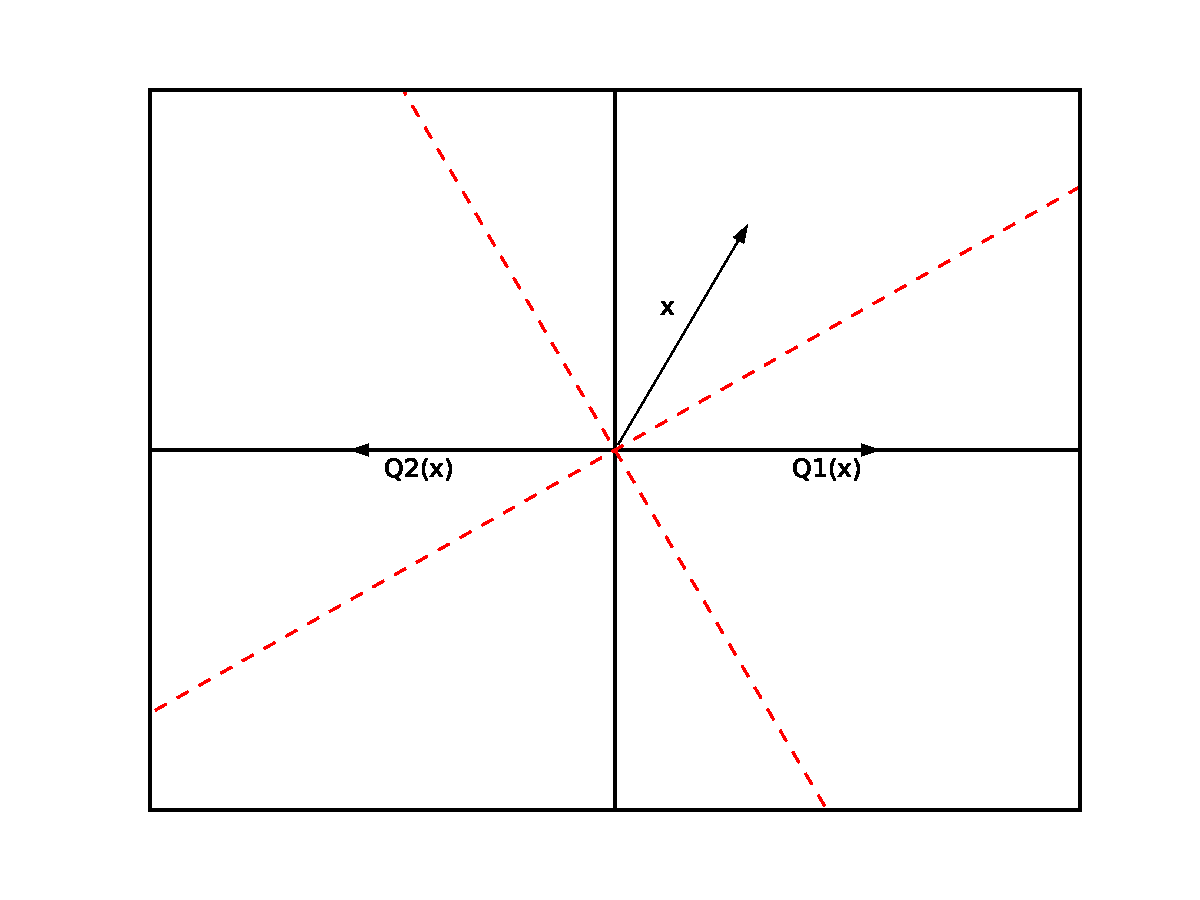
\includegraphics[width=7.5cm]{fig2}
%\end{array}$
\end{center}
\caption{A two-stage weight loss intervention for a 38 year old female, standing 5'8'' and weighing 160 lbs.  The first 16-week period corresponds to an aggressive weight loss stage, where intake is reduced from 2143 to 1600 calories/day and physical activity is increased from little to no exercise (PAL=1.4) to an hour of exercise 5 days per week (PAL=1.7).  The second 4-month period is achieved by increasing intake from 1600 to 2025 calories/day, and a decreasing exercise to 2-3 days per week (PAL=1.5).  The second period is the maintenance stage, which corresponds to a steady-state weight of 136 lbs.  The two horizontal dotted lines corresponds to the range given by a BMI of 20 and 25.  With this plan, the female subject would go from being on the high end of the normal weight range, to the low end.}
\label{first_simulation}
\end{figure}
%

In Figure \ref{first_simulation}, we see the weight curve of the woman in our ongoing example participating in a two-stage intervention.  This contrasts with the one-stage intervention in Figure \ref{second_simulation}, where the female subject takes a less aggressive but much lengthier approach.


\begin{figure}[t]
\begin{center}%$
%\begin{array}{lr}
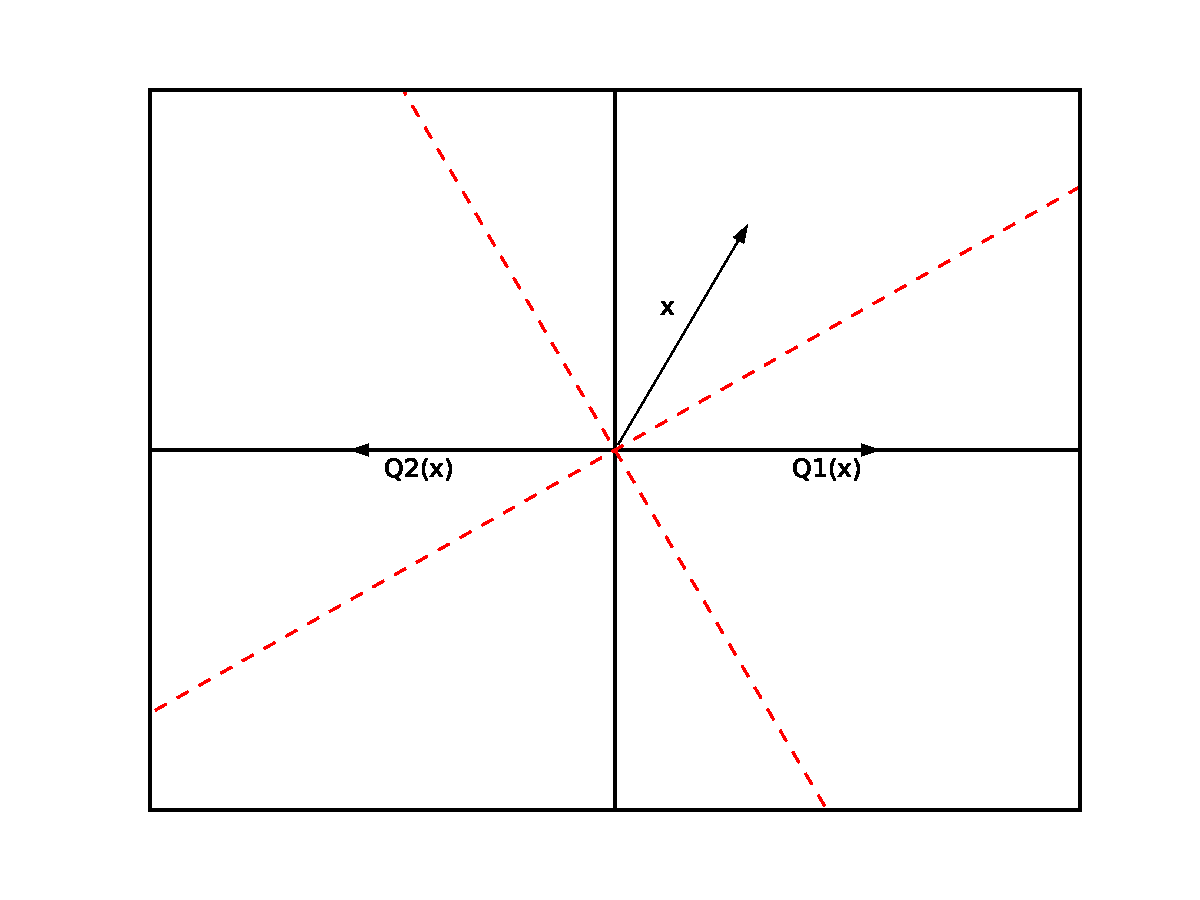
\includegraphics[width=12cm]{fig2} %&
%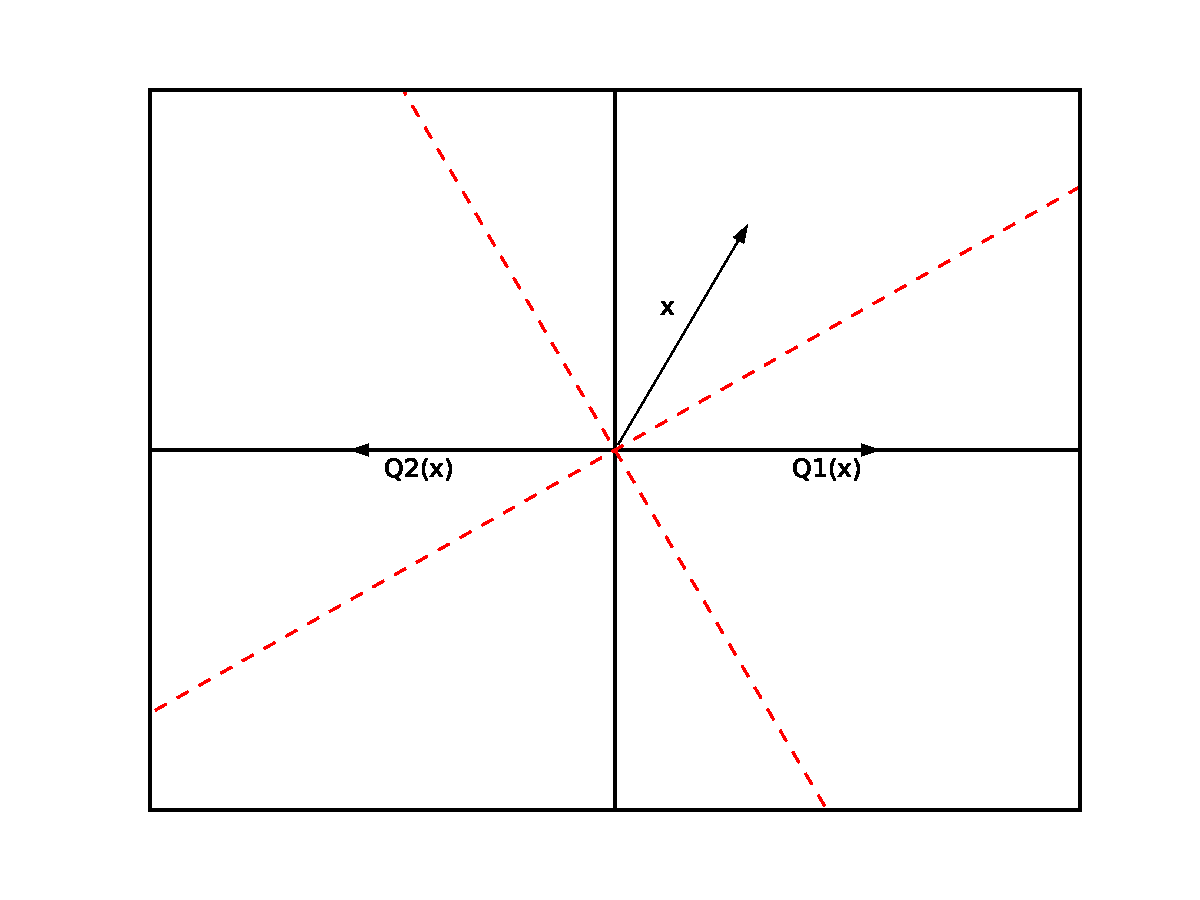
\includegraphics[width=7.5cm]{fig2}
%\end{array}$
\end{center}
\caption{A single-stage weight loss intervention for a 38 year old female, standing 5'8'' and weighing 160 lbs.  This 5-year curve corresponds to a long-term, but modest program, where intake is reduced from 2143 to 2025 calories/day, and physical activity from little to no exercise (PAL=1.4) to exercising to 2-3 days per week (PAL=1.5).  This approach also leads to a steady-state weight of 136 lbs after 5 years.  The two horizontal dotted lines corresponds to the range given by a BMI of 20 and 25.  With this plan, the female subject would go from being on the high end of the normal weight range, to the low end.}
\label{second_simulation}
\end{figure}

%%%%%%%%%%%%%%%%%%%%%%%%%%%%%%%%%%%%%%%%%%%
%%%%%%%%%%%%%%%%%%%%%%%%%%%%%%%%%%%%%%%%%%%
%%%%%%%%%%%%%%%%%%%%%%%%%%%%%%%%%%%%%%%%%%%

\section{Steady-State Calculations}

In this section, we determine the steady-state properties of a given intervention.  Before doing so, however, we first review the Lambert-$W$ function.

Consider the map $f(x) = x e^{x}$.  Since the derivative $f'(x) = (1+x) e^{x}$ is positive for $x>-1$, we have that $f$ is monotone, and thus invertible on the domain $[0,\infty)$.  We define the Lambert-$W$ function $\mathcal{W}$ to be the inverse.  Hence, $z = x e^{x}$ if and only if $x = \mathcal{W}[z]$.  We also have that $x = \mathcal{W}[x e^{x}]$, for all $x$ in the domain.  Computing the $\mathcal{W}[x]$ for a given $x$ is non-trivial.  One approach is to use Newton's method; there are other techniques as well (cite).  There are libraries available in C, Fortran, python, etc.  MATLAB has a built-in version of the function given by {\tt lambertw}.  Our first application of Lambert's function is given in the following:

\begin{lemma}
Consider the dynamical system \eqref{compartment} with equilibrium state $(F_i,L_I)$.  If the body weight changes by $\Delta BW$, then the new equilibrium state $(F_f,L_f)$ is given by
\begin{subequations}
\label{forbes_Ff}
\begin{align}
F_f &= C \cdot \mathcal{W}\left[ \dfrac{F_i}{C}\exp\left( \dfrac{\Delta BW + F_i}{C}\right)\right],\label{forbes_Ff:a}\\
L_f &= \Delta BW + F_i + L_i - F_f,\label{forbes_Ff:b}
\end{align}
\end{subequations}
where $C$ is the Forbes constant in \eqref{Forbes2}.
\end{lemma}

\begin{proof}
Since \eqref{forbes_Ff:b} is trivial, we only prove \eqref{forbes_Ff:a}. From Forbes' Law \eqref{Forbes}, we have that $F = D e^{L/C}$, where $D$ is a constant of integration.  Thus, we have that
\begin{subequations}
\label{F}
\begin{align}
F_i &= D \exp \left(\dfrac{L_i}{C}\right)\label{F:i},\\
F_f &= D \exp \left(\dfrac{L_f}{C}\right)\label{F:f}.
\end{align}
\end{subequations}
Combining \eqref{F:f} with \eqref{forbes_Ff:b} gives
\[
F_f = D \exp\left(\dfrac{\Delta BW + F_i + L_i - F_f}{C}\right).
\]
By simplifying, and using \eqref{F:i}, we have
\begin{equation}
\label{Ff2}
\dfrac{F_f}{C}  \exp \left(\dfrac{F_f}{C} \right)= \dfrac{F_i}{C} \exp\left(\dfrac{\Delta BW + F_i}{C}\right).
\end{equation}
Thus, taking the Lambert-$W$ function of both sides and simplifying, we have \eqref{forbes_Ff:a}.
\end{proof}

We now show how to compute the change in body weight $\Delta BW$ that comes from a long-term change in energy intake and physical activity.

\begin{theorem}
Consider the dynamical system \eqref{compartment} with equilibrium state $(F_i,L_I)$ and initial lifestyle $(EI_i,PAL_i)$.  If the subject's lifestyle changes to $(EI_f,PAL_f)$, then the steady-state change in body weight $\Delta BW$ is given by
\begin{equation}
\label{BW}
\Delta BW = \dfrac{\Phi}{\gamma_L} - F_i + \dfrac{C(\gamma_L-\gamma_F)}{\gamma_F}\cdot \mathcal{W}\left[\dfrac{\gamma_F}{\gamma_L}\cdot \dfrac{F_i}{C} \exp\left(\dfrac{\Phi}{\gamma_L C}\right) \right],
\end{equation}
where
\[
\Phi = \left(\dfrac{1}{PAL_f} - \dfrac{1}{PAL_i}\right) EI_i + \left(\dfrac{1}{PAL_f} - \beta_{AT}\right) \Delta EI + \gamma_F F_i.
\]
\end{theorem}

\begin{proof}
At equilibrium, we have
\[
\dfrac{EI_i}{PAL_i} = K + \gamma_F F_i + \gamma_L L_i + \beta_{AT} EI_i
\]
and
\[
\dfrac{EI_i + \Delta EI}{PAL_f} = K + \gamma_F F_f + \gamma_L L_f + \beta_{AT} EI_f.
\]
Subtracting, yields
\[
\Phi = \gamma_L (\Delta BW + F_i) + (\gamma_F-\gamma_L) F_f.
\]
Thus, we have that
\begin{equation}
\label{BW_temp}
\Delta BW = \dfrac{\Phi}{\gamma_L} - F_i + \dfrac{C(\gamma_L-\gamma_F)}{\gamma_F} \cdot \dfrac{\gamma_F F_f}{\gamma_L C}.
\end{equation}
Note that
\begin{align*}
\dfrac{\gamma_F F_f}{\gamma_L C} &= \mathcal{W}\left[ \dfrac{\gamma_F F_f}{\gamma_L C} \exp\left(\dfrac{\gamma_F F_f}{\gamma_L C}\right)\right]\\
&=  \mathcal{W}\left[\dfrac{\gamma_F}{\gamma_L}\cdot \dfrac{F_f}{ C} \exp\left(\dfrac{F_f}{C}\right)  \exp\left(\dfrac{(\gamma_F -\gamma_L)F_f}{\gamma_L C}\right) \right]\\
&=  \mathcal{W}\left[\dfrac{\gamma_F}{\gamma_L}\cdot  \dfrac{F_i}{C} \exp\left(\dfrac{\gamma_L(\Delta BW + F_i) +(\gamma_F -\gamma_L)F_f}{\gamma_L C}\right) \right]\\
&=  \mathcal{W}\left[\dfrac{\gamma_F}{\gamma_L}\cdot \dfrac{F_i}{C} \exp\left(\dfrac{\Phi}{\gamma_L C}\right) \right].
\end{align*}
Substituting this into \eqref{BW_temp} gives \eqref{BW}.
\end{proof}

%In the previous problem, we showed how to find $\Delta BW$ given a prescribed intervention $(EI,PAL)$.  We now show how to find $EI$ given a desired $BW$ and $PAL$.  First, we note that TODO.

%%%%%%%%%%%%%%%%%%%%%%%%%%%%%%%%%%%%%%%%%%%
%%%%%%%%%%%%%%%%%%%%%%%%%%%%%%%%%%%%%%%%%%%
%%%%%%%%%%%%%%%%%%%%%%%%%%%%%%%%%%%%%%%%%%%


%\section{Consequences of Dynamic Model}
%
%TODO: Talk about the recent models and the ability to tailor a model to a specific individual with RMR test with Korr.  Also, look at the following problems:
%\begin{itemize}
%\item What change in EB is necessary to achieve a certain weight by a certain date.
%\item How to deal with aging, and the drop in metabolism
%\item Extra-cellular fluid and how people change water weight according to carb and sodium variation
%\item Taking daily weight and backing out daily EB estimates
%\item Taking daily weight, EI and PAL and fine-tuning the model
%\end{itemize}
%
%Note long-observed exponential decay toward the equilibrium \cite{Fo.1}.
%
%A more detailed model is found in \cite{Hall.3}.

%There has been a recent growth in employer and community-outreach programs that use social networks and financial incentives to help promote healthy choices 
%\cite{Gr} -- More coaching means better results
%\cite{Vo} -- Incentives help with short-term behavior
%\cite -- Social networking in weight loss

\newpage
\appendix 



\section{Physical Activity Level: A Detailed Approach}
\label{PAL_appendix}

In this appendix, we show how to determine one's PAL based on a survey of physical activity for the day.  See \cite{Heym}.

\begin{table}[h]
\label{PAL_table}
\begin{center}
\begin{tabular}{|l|r|}
\hline
Daily & Physical Activity\\
Activities & Ratio (PAR)\\
\hline
Sleeping & 1.0 \\
Light Leisure (watching TV, lounging, chatting) & 1.4 \\
Sitting (eating, office work, meetings, computer) & 1.5 \\
Driving Car & 2.0 \\
Cooking & 2.1 \\
Personal Care (dressing, showering) & 2.3 \\
General Household Work & 2.8 \\
Walking (regular speed) & 3.2 \\
Low-Intensity Aerobics & 3.5 \\
Stairs & 5.0 \\
Biking & 5.6 \\
Running (long-distance) & 6.4 \\
High-Intensity Aerobics & 7.9 \\
Basketball & 8.0 \\
Swimming & 9.0 \\
\hline
\end{tabular}
\caption{}
\end{center}
\end{table}

\begin{table}[h]
\label{PAL_table2}
\begin{center}
\begin{tabular}{|l|r|r|r|}
\hline
Daily Activities & Time Allocation (h) & Energy Cost (PAR) & Time $\times$ Energy Cost \\
\hline
Sleeping & 8.0 & 1.0 & 8.0 \\
Personal Care & 1.0 & 2.3 & 2.3 \\
Eating & 1.0 & 1.5 & 1.5 \\
Cooking & 1.0 & 2.1 & 2.1 \\
Sitting (at work) & 8.0 & 1.5 & 12.0 \\
Household Work & 1.0 & 2.8 & 2.8 \\
Driving Car & 1.0 & 2.0 & 2.0 \\
Walking & 1.0 & 3.2 & 3.2 \\
Light Leisure Activities & 2.0 & 1.4 & 2.8 \\
\hline
Total & 24.0 & & 36.7 \\
\hline
\end{tabular}
\caption{The PAL for this regiment is $36.7/24.0 = 1.53$.}
\end{center}
\end{table}

%%%%%%%%%%%%%%%%%%%%%%%%%%%%%%%%%%%%%%%%%%%
%%%%%%%%%%%%%%%%%%%%%%%%%%%%%%%%%%%%%%%%%%%
%%%%%%%%%%%%%%%%%%%%%%%%%%%%%%%%%%%%%%%%%%%


\newpage
\bibliographystyle{unsrt}
%\bibliographystyle{unsrt-annote}
\bibliography{rfc}
\end{document}

%%%%%%%%%%%%%%%%%%%%%%%%%%%%%%%%%%%%%%%%%%%
%%%%%%%%%%%%%%%%%%%%%%%%%%%%%%%%%%%%%%%%%%%
%%%%%%%%%%%%%%%%%%%%%%%%%%%%%%%%%%%%%%%%%%%
%%%%%%%%%%%%%%%%%%%%%%%%%%%%%%%%%%%%%%%%%%%

%FOOTNOTE: Obesity Survival Paradox: In people with heart failure, those with a BMI between 30.0 and 34.9 had lower mortality than those with a normal weight. This has been attributed to the fact that people often lose weight as they become progressively more ill.[57] Similar findings have been made in other types of heart disease. People with class I obesity and heart disease do not have greater rates of further heart problems than people of normal weight who also have heart disease. In people with greater degrees of obesity, however, risk of further events is increased.[58][59] Even after cardiac bypass surgery, no increase in mortality is seen in the overweight and obese.[60] One study found that the improved survival could be explained by the more aggressive treatment obese people receive after a cardiac event.[61] Another found that if one takes into account chronic obstructive pulmonary disease (COPD) in those with PAD the benefit of obesity no longer exists.[56]
%Habbu A, Lakkis NM, Dokainish H (October 2006). "The obesity paradox: Fact or fiction?". Am. J. Cardiol. 98 (7): 944�8. doi:10.1016/j.amjcard.2006.04.039. PMID 16996880.
%^ Romero-Corral A, Montori VM, Somers VK, et al. (2006). "Association of bodyweight with total mortality and with cardiovascular events in coronary artery disease: A systematic review of cohort studies". Lancet 368 (9536): 666�78. doi:10.1016/S0140-6736(06)69251-9. PMID 16920472.
%^ Oreopoulos A, Padwal R, Kalantar-Zadeh K, Fonarow GC, Norris CM, McAlister FA (July 2008). "Body mass index and mortality in heart failure: A meta-analysis". Am. Heart J. 156 (1): 13�22. doi:10.1016/j.ahj.2008.02.014. PMID 18585492.
%^ Oreopoulos A, Padwal R, Norris CM, Mullen JC, Pretorius V, Kalantar-Zadeh K (February 2008). "Effect of obesity on short- and long-term mortality postcoronary revascularization: A meta-analysis". Obesity (Silver Spring) 16 (2): 442�50. doi:10.1038/oby.2007.36. PMID 18239657.
%^ Diercks DB, Roe MT, Mulgund J et al. (July 2006). "The obesity paradox in non-ST-segment elevation acute coronary syndromes: Results from the Can Rapid risk stratification of Unstable angina patients Suppress ADverse outcomes with Early implementation of the American College of Cardiology/American Heart Association Guidelines Quality Improvement Initiative". Am Heart J 152 (1): 140�8. doi:10.1016/j.ahj.2005.09.024. PMID 16824844.

